% !TEX root = ../main.tex

\chapter{Race-Averse Scheduler}

\section{RAS Introduction}

CPU scheduling is the basis of multiprogrammed operating systems. By switching the CPU among tasks, the operating system can make the computer more productive. In a single-processor system, only one task can run at a time. Others must wait until the CPU is free and can be rescheduled\cite{schedintro}. Through frequently scheduling and context switch, tasks can run in a concurrent manner. The role of the Linux scheduler is to select the next task to run and distribute the running time.

Linux implements several kinds of schedulers for different scheduling situation. For example, Linux has RT Scheduler for real-time tasks, CFS Scheduler for normal tasks and IDLE Scheduler for tasks with least importance. When these schedulers pick a task, they take a variety of factors into account. However, the likelihood that a task may race with other currently running tasks is not considered. Therefore, we propose a Race-Averse Scheduling (RAS) algorithm. The scheduling is a Weighted Round Robin style scheduling according to race probabilities of each running task.

\section{RAS Design}

\subsection{How RAS works}

First we will introduce the Weighted Round Robin scheduling. Round Robin scheduling treats all tasks equally. It distribute the same \textit{timeslice}\footnote{A concept in Linux Scheduling. Refers to a period of time for the task to run. Usually 10ms\textasciitilde100ms.} to every picked task. When a task runs out of its timeslice, it would yield the execution by its self, and be put back on the end of the \textit{run queue}\footnote{A concept in Linux Scheduling. Every task which is ready but not running will be waiting in the run queue for being picked to run.}. 

\begin{figure}[!htp]
  \centering
  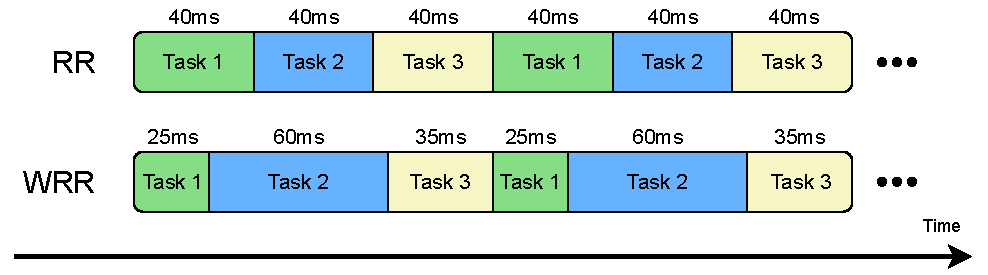
\includegraphics[width=12cm]{figures/wrr.drawio.pdf}
  \caption{Round Robin \& Weighted Round Robin}
\end{figure}

However, there are some situations where it is desirable to give some tasks preference over the others. That is, distributing longer timeslice to some tasks. Weighted Round Robin actually does this. The only difference between Round Robin and Weighted Round Robin is that Weighted Round Robin will assign a weight to each task, and tasks with higher weights will be given longer timeslice to run.

Obviously, in Race-Averse Scheduler, the weights are determined by the race probabilities. In our design, the race probability of a task is represented as an integer in the range of [0, 10). The higher the integer is, the more likely that the task may race with others. For CPU, it is rational to give preference to the tasks with lower race probabilities. That is exactly what the Race-Averse means. Therefore, tasks with lower race probabilities will be assigned with higher weights, which is, with longer timeslice to run. 

With the assistance of the Memory Access Tracing we implemented before, we can quantify the race probabilities between different running tasks. To simplify the situation, we assume that a large enough number of tasks are in scheduling, and they may compete at a given range of virtual addresses. Thus, the race probability of a certain task is proportional to its frequency of accessing the given range of virtual addresses. We can use the following equation to calculate the race probability:

\begin{equation}
    race\_prob_i = 10\times\frac{wcounts_i}{\sum_{i}wcounts_i}
\end{equation}

We set the maximum timeslice of the Race-Averse Scheduler to 100ms and the minimum timeslice to 10ms. And we can inversely map the race probabilities from 0 to 9 into the timeslice from 100ms to 10ms:


\begin{equation}
\begin{aligned}
    timeslice &= \frac{max\_timeslice-min\_timeslice}{0-9}\times race\_prob+max\_timeslice\\
    &= -10ms\times race\_prob + max\_timeslice
\end{aligned}
\end{equation}

When a task runs out of its timeslice, the RAS will compute the sum of \textit{wcounts} of the tasks in RAS run queue, and further calculate its race probability. Then assign a new timeslice according to its race probability, and put the task back to the end of the run queue. We should notice that the weight of a task can be changed dynamically, due to the newly coming tasks, completed tasks and some other reasons. Therefore, we have to re-compute the race probability every time the task needs to be assigned with new timeslice.

\subsection{Into Linux Kernal}

Now we are familiar with how the Race-Averse Scheduler works. Next, we will look into the Linux kernel and introduce how to embed the Race-Averse Scheduler into the kernel.

There are many ready tasks waiting for running in kernel. To manage these tasks, the kernel maintains a \textit{Run Queue} of these tasks. Besides, we call the task that the CPU is running \textit{Current Task}. To switch different tasks to Current Task, first the kernel should set the \textit{Need Resched} flag to Current Task, and second the kernel should check the Need Resched flag at a proper time. If Current Task needs to be rescheduled, the kernel calls \textit{Schedule} function to perform a context switch. The proper time actually refers to the time when CPU is interrupted by the ticker timer and etc. 

The Schedule function picking the next task needs the help of \textit{Scheduling Class}. Linux uses Scheduling Class to implement different scheduling algorithms. Here we take \textit{rt\_sched\_class}\footnote{\textit{rt\_sched\_class} implements FIFO and RR scheduling algorithms.}, \textit{cfs\_sched\_class}\footnote{\textit{cfs\_sched\_class} implements Completely Fair Scheduling algorithm.}, \textit{idle\_sched\_class}\footnote{\textit{idle\_sched\_class} implements IDLE scheduling algorithm.} and our \textit{ras\_sched\_class} as example. These classes are linked together through a linked list. When Schedule function wants to pick the next task, it will iterate through the schedule classes linked list and try to get a task from their own run queues. Once it gets a valid task, it would return directly and set the task as Current Task. So it is easy to see that every schedule class has different priorities. The head class of the linked list has higher priority than the tail class. Only when the former class doesn't have any task in run queue, the current class can pick its task in its run queue to return. Therefore, if we make different queue arrangement rules for different schedule classes, the tasks can be scheduled with different scheduling algorithms. For example, the run queue of \textit{rt\_sched\_class} contains multi priorities queues, and the run queue of \textit{cfs\_sched\_class} is a Red-Black Tree. From our previous discussion, we can learn that the run queue of RAS is a simple single queue.

\begin{figure}[!htp]
  \centering
  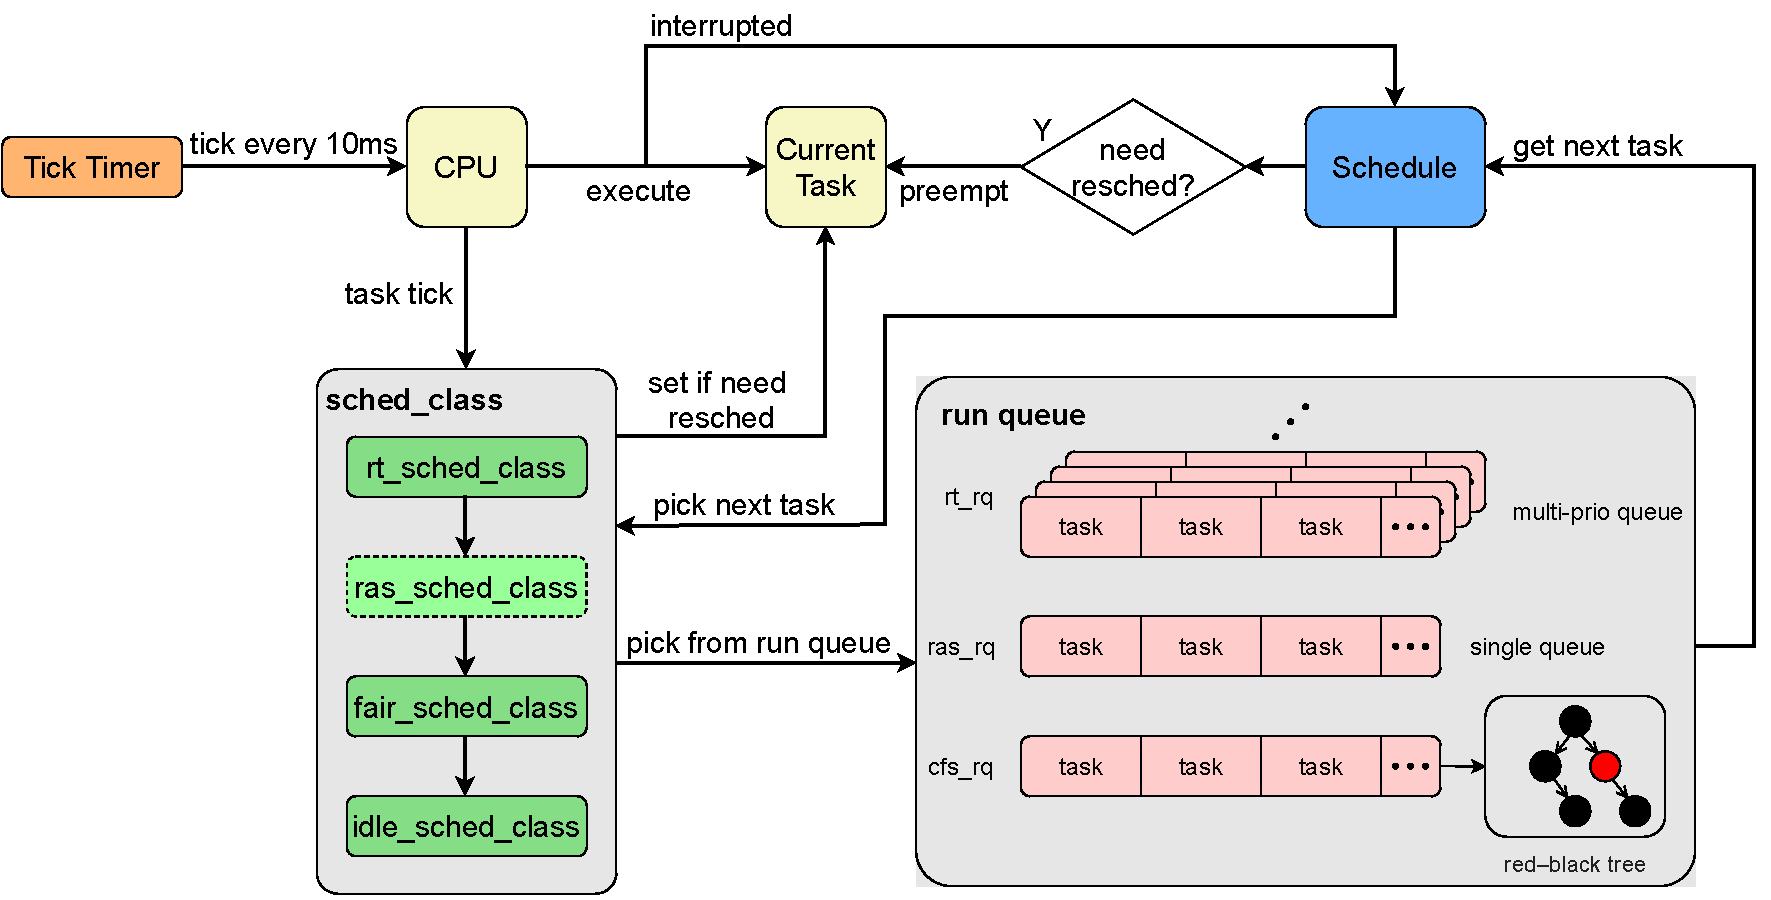
\includegraphics[width=14cm]{figures/scheduler.drawio.pdf}
  \caption{Linux Scheduling Procedure}
\end{figure}

Therefore, what we really need to implement is a new schedule class, \textit{ras\_sched\_class}.

\section{RAS Implementation}

The Scheduler Class has the following structure:

\begin{codeblock}[language=C]
// include/linux/sched.h
struct sched_class {
	const struct sched_class *next;
	void (*enqueue_task) (struct rq *rq, struct task_struct *p, int flags);
	void (*dequeue_task) (struct rq *rq, struct task_struct *p, int flags);
	struct task_struct* (*pick_next_task) (struct rq *rq);
	void (*task_tick) (struct rq *rq, struct task_struct *p, int queued);
	...
};
\end{codeblock}

All the scheduler classes should implement these functions. Their roles are closely related to the scheduling procedure of Linux Scheduler introduced above.

\begin{itemize}
    \item \textbf{\textit{next}}: points to the next scheduler class in the linked list. In our design, the next scheduler of RAS is Fair Scheduler, and the former scheduler of RAS is RT Scheduler.
    \item \textbf{\textit{enqueue\_task}}: enqueue a task into the run queue. 
    \item \textbf{\textit{dequeue\_task}}: dequeue a task from the run queue.
    \item \textbf{\textit{pick\_next\_task}}: pick a task from the run queue to be the next Current Task.
    \item \textbf{\textit{task\_tick}}: invoked when the tick timer ticks. Update some variables.
\end{itemize}

These four functions are the most important functions that we should implement for our Race-Averse Scheduler. Before implement these functions, we will define some structures associated with RAS.

\begin{figure}[!htp]
  \centering
  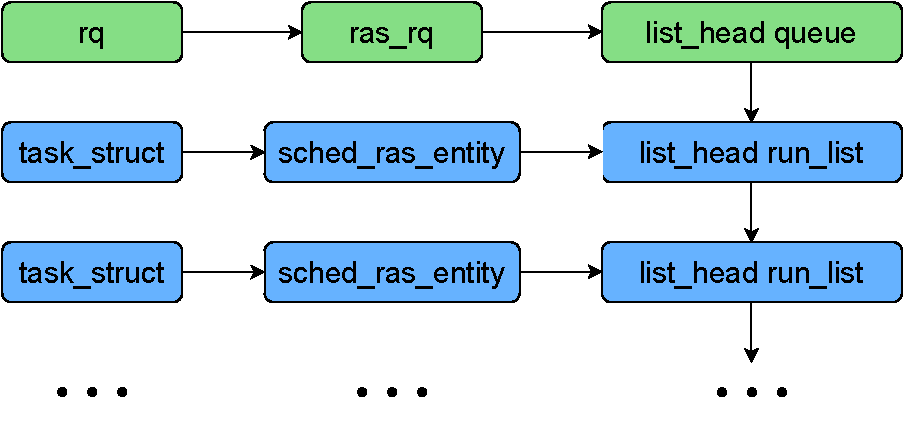
\includegraphics[width=11cm]{figures/structures.drawio.pdf}
  \caption{RAS Structures}
\end{figure}

\subsection{Structure ras\_rq}

Structure \textit{ras\_rq} is the implementation of the run queue of RAS. 

\begin{codeblock}[language=C]
// kernel/sched/sched.h
struct ras_rq 
{
	struct list_head queue;
	unsigned long ras_nr_running;
};
\end{codeblock}

\begin{itemize}
    \item \textbf{\textit{queue}}: the head of the RAS run queue linked list.
    \item \textbf{\textit{ras\_nr\_running}}: the number of tasks in RAS run queue.
\end{itemize}

\subsection{Structure sched\_ras\_entity}

Structure \textit{sched\_ras\_entity} represents an entity which can be scheduled by RAS, in other words, a task with the RAS scheduling strategy. Therefore, we should add a \textit{sched\_ras\_entity} variable in the \textit{task\_struct}.

\begin{codeblock}[language=C]
// include/linux/sched.h
struct sched_ras_entity 
{
	struct list_head run_list;
	unsigned int time_slice;
	unsigned int total_timeslice;
};
\end{codeblock}

\begin{itemize}
    \item \textbf{\textit{run\_list}}: the node in the RAS run queue linked list.
    \item \textbf{\textit{time\_slice}}: the timeslice left to run.
    \item \textbf{\textit{total\_timeslice}}: the timeslice allocated in this round.
\end{itemize}

With these structures defined, we can implement our RAS functions.

\subsection{Function enqueue\_task\_ras}

When a new task with RAS scheduling strategy comes into the kernel, or a task was switched from other scheduling strategy to RAS, the kernel will invoke \textit{enqueue\_task\_ras} to put the task into the RAS run queue.

\begin{codeblock}[language=C]
// kernel/sched/ras.c
static void
enqueue_task_ras(struct rq *rq, struct task_struct *p, int flags)
{
	struct sched_ras_entity *ras_se = &p->ras;
	struct ras_rq *ras_rq = &rq->ras;
	struct list_head *queue = &ras_rq->queue;
	list_add_tail(&ras_se->run_list, queue);
	ras_rq->ras_nr_running++;
	inc_nr_running(rq);
}
\end{codeblock}

We add the \textit{sched\_ras\_entity} to the tail of RAS run queue, and increase the count of running tasks.

\subsection{Function dequeue\_task\_ras}

When a task with RAS scheduling strategy finishes its job, or a task was switched from RAS to other scheduling strategy, the kernel will invoke \textit{dequeue\_task\_ras} to remove the task from the RAS run queue.

\begin{codeblock}[language=C]
// kernel/sched/ras.c
static void
dequeue_task_ras(struct rq *rq, struct task_struct *p, int flags)
{
	struct sched_ras_entity *ras_se = &p->ras;
	struct ras_rq *ras_rq = &rq->ras;
	list_del_init(&ras_se->run_list);
	ras_rq->ras_nr_running--;
	dec_nr_running(rq);
}
\end{codeblock}

We delete the \textit{sched\_ras\_entity} from RAS run queue, and decrease the count of running tasks.

\subsection{Function pick\_next\_task\_ras}

When the Scheduler function in the kernel wants to pick a task from the RAS run queue, \textit{pick\_next\_task\_ras} function will be called. It returns a task in the RAS run queue if there was.

\begin{codeblock}[language=C]
// kernel/sched/ras.c
static struct task_struct *
pick_next_task_ras(struct rq *rq)
{
	struct sched_ras_entity *ras_se;
	struct task_struct *p;
	struct ras_rq *ras_rq = &rq->ras;
	if (!ras_rq->ras_nr_running){
	  // No task in run queue, return null.
		return NULL;
	}
	struct list_head *queue = &ras_rq->queue;
	ras_se = list_entry(queue->next, struct sched_ras_entity, run_list);
	p = ras_task_of(ras_se);
	return p;
}
\end{codeblock}

The \textit{pick\_next\_task\_ras} function will select the head node of the run queue linked list to return. And if there is no task in run queue, it will return null.

\subsection{Function task\_tick\_ras}

The \textit{task\_tick\_ras} function is the most vital function for implementing Race-Averse Scheduler. In this function, we will compute the race probability of a task and dynamically allocate the task with some timeslice according to its race probability with other running tasks.

\begin{codeblock}[language=C]
// kernel/sched/ras.c
static void
task_tick_ras(struct rq *rq, struct task_struct *task, int queued)
{
	struct sched_ras_entity *ras_se = &task->ras;
	struct ras_rq *ras_rq = &rq->ras;
	if (task->policy != SCHED_RAS)
		return;		
	if (--task->ras.time_slice)
		return;
	if (ras_rq->ras_nr_running == 1){
		// No race. Set MAX timeslice to avoid frequently schedule.
		task->ras.time_slice = RAS_MAX_TIMESLICE;
		task->ras.total_timeslice = RAS_MAX_TIMESLICE;
	} else {
		// Calculate race probability.
		int wcounts = task->wcounts;
		struct list_head *p;
		struct sched_ras_entity *ras_se_tmp;
		struct task_struct *t;
		struct list_head *queue;
		queue = &ras_rq->queue;
		int sum = 0;
		int task_cnt = 0;
		list_for_each(p, queue)
		{
			ras_se_tmp = list_entry(p, struct sched_ras_entity, run_list);
			t = ras_task_of(ras_se_tmp);
			sum += t->wcounts;
			task_cnt++;
		}
		if (sum == 0 || sum == wcounts) {
			// not tracing or no memory write
			task->ras.time_slice = RAS_MAX_TIMESLICE;
			task->ras.total_timeslice = RAS_MAX_TIMESLICE;
		} else {
			int race_prob = wcounts * 10 / sum;
			unsigned int timeslice = -1*race_prob + RAS_MAX_TIMESLICE;
			task->ras.time_slice = timeslice;
			task->ras.total_timeslice = timeslice;
		}
	}
	
	// Requeue to the end of queue if we are NOT the only element on the queue.
	if (ras_se->run_list.prev != ras_se->run_list.next){
        requeue_task_ras(rq, task, 0);
        set_tsk_need_resched(task);
    }
}
\end{codeblock}

The \textit{task\_tick\_ras} function will be invoked every time the tick timer ticks. The tick timer ticks every 10ms. If the task has timeslice left, the function reduces its timeslice by one. If the task has no timeslice left, it indicates that the task should yield the CPU and be re-queued back to the tail of the run queue. Before the task is re-queued, it will be allocated with a new timeslice. If the task isn't being traced by Memory Access Tracer, or there is no memory write or task race, it will be allocated with the maximum timeslice. Otherwise, we iterate the tasks in the run queue and compute the race probability of the current task. Then allocate the timeslice according to its race probability.

\subsection{Some other functions}

With the four functions mentioned before, we can archive the basic operations of Race-Averse Scheduler. But we still need some other functions to implement the whole operations of RAS.

\begin{enumerate}
    \item \textit{\textbf{yield\_task\_ras}}: when the task wants to yield the CPU, this function will be called.
    \begin{codeblock}[language=C]
static void
yield_task_ras(struct rq *rq)
{
    requeue_task_ras(rq, rq->curr, 0);
}
    \end{codeblock}
    \item \textit{\textbf{update\_curr\_ras}}: update some statistical information of CPU and tasks.
    \begin{codeblock}[language=C]
static void update_curr_ras(struct rq *rq)
{
    struct task_struct *curr = rq->curr;
    struct sched_ras_entity *ras_se = &curr->ras;
    struct ras_rq *ras_rq = &rq->ras;
    u64 delta_exec;
    if (curr->sched_class != &ras_sched_class)
        return;
    delta_exec = rq->clock_task - curr->se.exec_start;
    if (unlikely((s64)delta_exec < 0))
        delta_exec = 0;
    schedstat_set(curr->se.statistics.exec_max,
	    		  max(curr->se.statistics.exec_max, delta_exec));
    curr->se.sum_exec_runtime += delta_exec;
    curr->se.exec_start = rq->clock_task;
}
    \end{codeblock}
    \item \textit{\textbf{put\_prev\_task\_ras}}: called before another task replaces the current task. For some statistical information.
    \begin{codeblock}[language=C]
static void
put_prev_task_ras(struct rq *rq, struct task_struct *p)
{
   	update_curr_ras(rq);
}
    \end{codeblock}
    \item \textit{\textbf{set\_curr\_task\_ras}}: called when the scheduling policy of the current task changes to RAS. For some statistical information.
    \begin{codeblock}[language=C]
static void
set_curr_task_ras(struct rq *rq)
{
	struct task_struct *p = rq->curr;
	p->se.exec_start = rq->clock_task;
}
    \end{codeblock}
    \item \textit{\textbf{get\_rr\_interval\_ras}}: return the total timeslice allocated before. For system calls.
    \begin{codeblock}[language=C]
static unsigned int
get_rr_interval_ras(struct rq *rq, struct task_struct *task)
{
	if (task->policy == SCHED_RAS)
	{
		struct sched_ras_entity *ras_se = &task->ras;
		return ras_se->total_timeslice;
	}
	return 0;
}
    \end{codeblock}
\end{enumerate}

Besides these structures and functions, we also have to re-write some code in the kernel source code to apply RAS to the kernel. For example, declare some variables and add some branch conditions of RAS. Please refer to the source code for detailed modification.

\section{RAS Test}

In this section, we write some test programs to check that whether RAS works correctly.

\subsection{Switch Test}

First, we launch a infinite loop program and get its \textit{pid}. Second, we use another program to change its scheduling policy to RAS, and then try to change back. Output information:

\begin{figure}[!htp]
  \centering
  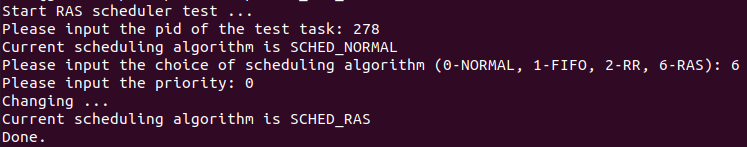
\includegraphics[width=12cm]{figures/basictest1.png}
  \caption{Change to RAS Policy}
  \label{fig:basictest1}
\end{figure}

\begin{figure}[!htp]
  \centering
  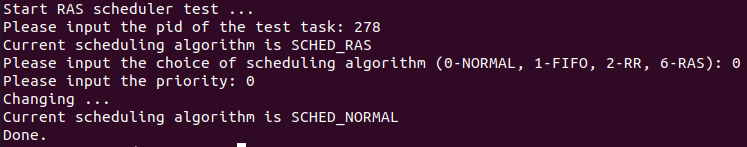
\includegraphics[width=12cm]{figures/basictest2.png}
  \caption{Change Back to NORMAL Policy}
  \label{fig:basictest2}
\end{figure}

In Figure~\ref{fig:basictest1} we can see that the task with pid 278 is successfully changed with the RAS policy. In Figure~\ref{fig:basictest2} we can see that it can also be changed back with the NORMAL policy. This proves that RAS is successfully embedded into Linux kernel.

\subsection{Multi-Tasks Test}

Now we write a test program to fork 10 child tasks and set their scheduling policy as RAS. Each task will write random times [128, 1024) to a given range of memory which is traced. Then we will check that RAS can whether correctly arrange their executions and allocate them with different timeslices according to their race probabilities. Output information is as following:

\begin{figure}[!htp]
  \centering
  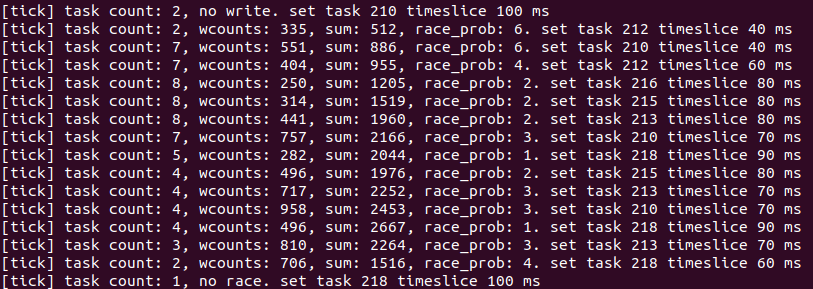
\includegraphics[width=13cm]{figures/multasktest1.png}
  \caption{RAS Multi Tasks Test Result}
  \label{fig:multitasktest}
\end{figure}

In Figure~\ref{fig:multitasktest} we can see that the RAS correctly scheduled these tasks in a weighted round robin style. When a task run out of its timeslice, it will be allocated with a new timeslice according to its race probability. Then it will be re-queued to the tail of the run queue. And RAS will pick the first task in the run queue as the next task to run.

These results prove that we successfully implemented the Race-Averse Scheduler.